\documentclass[12pt,a4paper,english,nofootinbib,sort&compress,numbers]{revtex4-2} % Defines the basic parameters of the document
% If you want a doubble-column, add "reprint"

% Allows special characters (including æøå)
\usepackage[utf8]{inputenc}

% It may be usefult to download TeXMaker, because it includes a large library of the most common packages.

\usepackage{physics,amssymb}  % mathematical symbols (physics imports amsmath)
\usepackage{amsmath}          %Allows usage of mathematical expressions
\usepackage{graphicx}         % include graphics such as plots
\graphicspath{ {Images/} }

\usepackage{xcolor}           % set colors
\usepackage{hyperref}         % automagic cross-referencing
\usepackage{listings}         % display code

\usepackage{algorithm}        % structure and display algorithms
\usepackage[noend]{algpseudocode} % environment to write pseudocode
\usepackage{float}            % make sure that algorithms float with revtex4-2
\usepackage{tikz}             % for creating graphics
% Defines the color of hyperref objects
% Blending two colors:  blue!80!black  =  80% blue and 20% black
\hypersetup{ % this is just my personal choice, feel free to change things
    colorlinks,
    linkcolor={red!50!black},
    citecolor={blue!50!black},
    urlcolor={blue!80!black}}


\usepackage{caption}          %Allows usage of plots
\usepackage{subcaption}       %Allows usage of subplots

\newcommand{\iris}[1]{\textbf{\textcolor{blue}{#1}}}
\newcommand{\jonas}[1]{\textbf{\textcolor{red}{#1}}}

\newcommand{\nl}{\bigskip\noindent}


\begin{document}
% ===========================================
% Title and authors
\title{FYS-STK4155 Project 1 \\ Comparison of the Linear regression models OLS, Ridge and Lasso}       
\author{Iris Bore, Lars-Martin Gihle \& Jonas Båtnes   \\ \textit{University of Oslo, Department of Physics}}   % Sets the author's name.
\date{\today}                  % Sets the document date.

% ===========================================

\noaffiliation                 % Ignore this, but keep it.

\begin{abstract}
    
\end{abstract}

\maketitle

% ===========================================
\section{Abstract}
%
\label{sec:Abstract}
 A significant amount of big data is geospatial data, and the size of such data is growing\cite{geospatital}. As big datasets become more common in geospatial analysis, it's important to assess how well standard linear regression methods work in these complex situations. Tests using synthetic data might not reveal the challenges posed by real-world data structures.  This study examines how three key linear regression methods perform when applied to different types of data: real-world high-dimensional topographic data and synthetic data generated from a uniform distribution. Our goal is to understand how these models behave under different conditions, such as adding constraints or changing the degrees of freedom. Our results show significant differences in model performance when applied to real-world data compared to synthetic data, especially concerning computational complexity and the influence of the data's structure. These findings highlight the difficulties of working with high-dimensional, real-world datasets and suggest that tailored approaches may be needed in these cases. \cite{openai2023chatgpt}

% ===========================================
% ===========================================
\newpage
\section{Introduction}
%
\label{sec:introduction}
In statistics and machine learning, regression analysis is a fundamental tool for modeling and understanding relationships within data \cite{hastie2009elements}. Ordinary Least Squares (OLS), Ridge Regression, and Lasso Regression are pivotal techniques that address challenges such as overfitting and high dimensionality, each providing unique insights into data structures \cite{hoerl1970ridge}\cite{tibshirani1996lasso}.
\newline

High-dimensional, real-world datasets like topographic terrain data present significant challenges related to computational complexity and intricate data patterns \cite{bellman1961adaptive}. To evaluate model performance and study the bias-variance tradeoff in such contexts, resampling methods like Bootstrap and K-fold cross-validation are essential \cite{efron1993bootstrap}\cite{arlot2010survey}. These techniques ensure robust model evaluation and enhance the generalizability of results.
\newline

In this study, we apply OLS, Ridge, and Lasso regression methods to both real terrain data and uniformly distributed synthetic data. By comparing the Mean Squared Error (MSE) and R-squared (R²) metrics across these datasets, we aim to understand how each regression method performs under varying data conditions. We also utilize Bootstrap and K-fold cross-validation to examine the bias-variance tradeoff and to find the optimal regularization parameter lambda and polynomial degree for Ridge and Lasso regression.
\newline 

The report is structured as follows. We begin by introducing the data generation and preprocessing. Next, we describe the regression techniques and resampling methods used in this study. Further, we describe the experimental setup, detailing how the models were validated and evaluated. We then present and discuss our findings, focusing on model performance metrics and the reproduction of terrain data based on K-fold cross-validation. Finally, we summarize our conclusions and suggest directions for future research.


% ===========================================
\newpage
\section{Methods}\label{sec:methods}
%
\label{sec:methods}
In this study, we employed several machine learning techniques to model and analyze the synthetic terrain data generated by the Franke Function. The primary focus was on implementing and comparing the performance of Ordinary Least Squares (OLS), Ridge regression, and Lasso regression. To ensure the robustness and reliability of our results, we utilized data preprocessing techniques and validation methods, including train-test splitting, feature scaling, cross-validation, and bootstrapping.

\subsection{Data Generation and Preprocessing}

The synthetic dataset was generated using the Franke Function equation \ref{eq:frankefunction} over a grid of $(x, y)$ values from the uniform distribution. To simulate real-world data imperfections, normally distributed noise was added to the output $f(x, y)$. We used the seed "2024" to create consistent data. The resulting dataset was then prepared for regression analysis. The real terrain data was taken from the file \texttt{SRTM\_data\_Norway\_1.tif} from the course datafiles \cite{CompPhysics2023}.

\begin{equation}
\begin{split}    
    f(x, y) = & \ \frac{3}{4} e^{-\frac{(9x-2)^2}{4} - \frac{(9y-2)^2}{4}} + \frac{3}{4} e^{-\frac{(9x+1)^2}{49} - \frac{(9y+1)}{10}} \\
    & + \frac{1}{2} e^{-\frac{(9x-7)^2}{4} - \frac{(9y-3)^2}{4}} - \frac{1}{5} e^{-(9x-4)^2 - (9y-7)^2}
   \label{eq:frankefunction}
\end{split}
\end{equation}

\subsubsection{Train-Test Split}

To evaluate the predictive performance of the models, the dataset was split into training and testing sets using the \texttt{train\_test\_split} function from the \texttt{scikit-learn} library \cite{scikit-learn}. The data was partitioned such that 80\% was used for training and 20\% for testing. This split ensures that the models are trained on a substantial portion of the data while reserving a separate set for unbiased evaluation.

\subsubsection{Feature Scaling}

Feature scaling is crucial for algorithms that are sensitive to the magnitude of the features, especially when regularization is involved. Without scaling, the features with larger values will be penalized more than those with small values. We scaled the variables using the \texttt{StandardScaler} from \texttt{scikit-learn}. Standardization transforms the data to have zero mean and unit variance, computed as:

\begin{equation}
    z = \frac{x - \mu}{\sigma}
\end{equation}

where $x$ is the original feature value, $\mu$ is the mean, and $\sigma$ is the standard deviation of the feature values in the training set. By centering the data, we reduce the multicollinearity of the columns with higher power in the design matrix. This makes our model more numerically stable. It can also reduce the risk of our design-matrix becoming nearly-singular, which makes computation easier.\cite{polyreg_budescu}

A downside with using the standard scaler is that it doesn´t provide a minimum and a maximum value for our data set. \cite{Hjorth-Jensen_MachineLearning_2023} However, it is both really easy to understand and easy to implement, which we weighed more.

The scaler was fit on the training data and then applied to both training and test sets to prevent data leakage between the two. When using cross-validation later on, we should ideally have scaled the data in each fold \ref{algo:kfold} for the same reason, but for simplicity and consistency of our code, we decided against it. 

 Although real data often benefits more from scaling than "perfect" data generated from a uniform distribution with mean zero, we scaled both the synthetic data and the terrain data to be consistent throughout the project. When trying to recreate our real data later on, we had to do an inverse scaling to get the correct values. 


\subsection{Regression Techniques}

The following regression techniques were implemented:

\subsubsection{Ordinary Least Squares (OLS)}

OLS served as the baseline model without regularization, optimized by minimizing the residual sum of squares in equation \ref{eq:betaOLS}. The model was fitted using the closed-form solution provided by the normal equation.

\begin{equation}
    \boldsymbol{\beta}_{\text{OLS}} = (\mathbf{X}^T \mathbf{X})^{-1} \mathbf{X}^T \mathbf{y}
    \label{eq:betaOLS}
\end{equation}

\subsubsection{Ridge Regression}

Ridge regression introduces an $L2$ penalty term to shrink the coefficients, controlled by a regularization parameter $\lambda$. The objective function to minimize equation \ref{eq:Ridgeminimize}.

\begin{equation}
       \text{Ridge:} \quad \min_{\boldsymbol{\beta}} \left\{ \sum_{i=1}^{n} (y_i - \hat{y}_i)^2 + \lambda \sum_{j=1}^{p} \beta_j^2 \right\}
    \label{eq:Ridgeminimize}
\end{equation}

where $\lambda$ is the regularization parameter, and $p$ is the number of predictors. The solution for the Ridge regression coefficients is as described in equation \ref{eq:betaRidge}:

\begin{equation}
    \boldsymbol{\beta}_{\text{Ridge}} = (\mathbf{X}^T \mathbf{X} + \lambda \mathbf{I})^{-1} \mathbf{X}^T \mathbf{y}
    \label{eq:betaRidge}
\end{equation}

We used grid search combined with 20-fold cross-validation to find the optimal value of $\lambda$. The search spanned a range of $\lambda$ values on a logarithmic scale to capture both small and large regularization effects.

\subsubsection{Lasso Regression}
\begin{figure}[h]
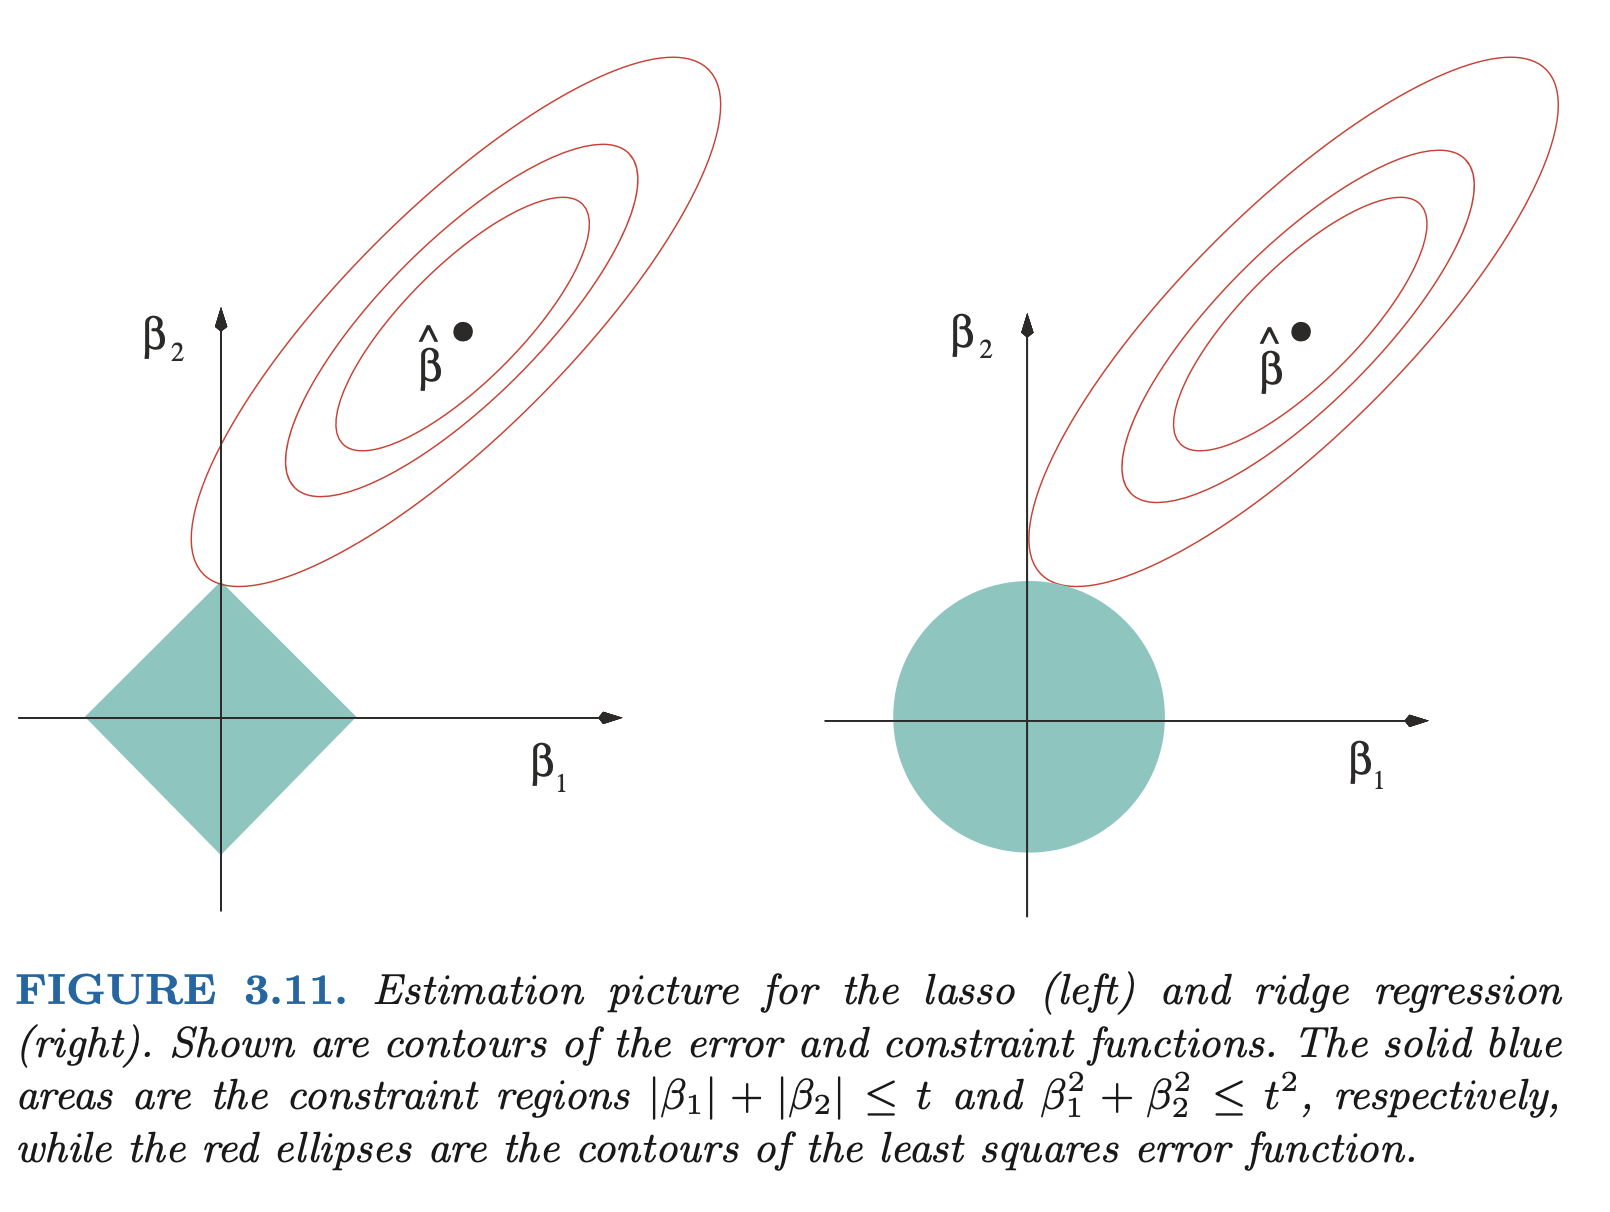
\includegraphics[width=8cm]{method_ridge_vs_lasso.png}
\caption{We have here borrowed figure 3.11 from ESL to illustrate the difference between how the L1 and L2 norm shrinks the parameters. \cite{ESL}}
\label{fig:L1vsL2}
\end{figure}

Lasso regression incorporates an $L1$ penalty to promote sparsity in the coefficients, controlled by the regularization parameter $\lambda$. The objective was to miminize beta in equation \ref{eq:Lassominimize}. 

\begin{equation}
    \text{Lasso:} \quad \min_{\boldsymbol{\beta}} \left\{ \sum_{i=1}^{n} (y_i - \hat{y}_i)^2 + \lambda \sum_{j=1}^{p} |\beta_j| \right\}
    \label{eq:Lassominimize}
\end{equation}

From figure \ref{fig:L1vsL2} we see that the constraint region imposed by $L1$ (left) makes it more likely that the optimal $\beta$ (where the OLS estimate $\hat{\beta}$ meets the constraint region) is zero, than for Ridge regression (right). 

Similar to Ridge regression, we used grid search and 10-fold cross-validation to select the optimal $\lambda$. The $L1$ penalty tends to set some coefficients exactly to zero, effectively performing feature selection.

\subsubsection{Expectation and variance in linear regression}
In the context of ordinary least squares (OLS), the vector of observations $( \mathbf{y} )$ is modeled as:
$$\mathbf{y} = \mathbf{X} \boldsymbol{\beta} + \boldsymbol{\epsilon}$$
For each element $( y_i )$ in the vector $( \mathbf{y} )$, we have:
$$y_i = \sum_j x_{ij} \beta_j + \epsilon_i$$
where $( x_{ij} )$ is the element in the $( i )-th$ row and $( j )-th$ column of the matrix $( \mathbf{X} )$, and $( \epsilon_i )$ is the corresponding error for the $( i )-th$ observation.
We then take the expectation of $y_i$.
$$\mathbb{E}(y_i) = \mathbb{E}\left( \sum_j x_{ij} \beta_j + \epsilon_i \right)$$
By the linearity of expectation, we have that:
$$\mathbb{E}(y_i) = \sum_j x_{ij} \beta_j + \mathbb{E}(\epsilon_i)$$
Since $( \epsilon_i )$ is normally distributed with mean 0, we have:
$$\mathbb{E}(\epsilon_i) = 0$$
$$\mathbb{E}(y_i) = \sum_j x_{ij} \beta_j$$
In matrix form, this can be written as:
$$\mathbb{E}(y_i) = \mathbf{X}_{i,*} \boldsymbol{\beta}$$
where $( \mathbf{X}_{i,*} )$ is the $( i )-th$ row of the design matrix $( \mathbf{X} )$
Thus the expectation value of $( y_i )$ is:
$$\mathbb{E}(y_i) = \sum_j x_{ij} \beta_j = \mathbf{X}_{i,*} \boldsymbol{\beta}$$

We then find the variance
$$\text{Var}(y_i) = \text{Var}\left(\sum_j x_{ij} \beta_j + \epsilon_i\right)$$

Since the deterministic part $( \sum_j x_{ij} \beta_j )$ is constant with respect to the random error $( \epsilon_i )$, its variance is 0. Thus, we have:

$$\text{Var}(y_i) = \text{Var}(\epsilon_i)$$

From the assumptions, we know that $(\epsilon_i \sim N(0, \sigma^2))$, so:

$$\text{Var}(\epsilon_i) = \sigma^2$$

Thus, we can then conclude that:

$$\text{Var}(y_i) = \sigma^2$$

The OLS estimator for the regression coefficients $( \hat{\beta} )$ is given by the well-known formula:

$$\hat{\beta} = (\mathbf{X}^\top \mathbf{X})^{-1} \mathbf{X}^\top \mathbf{y}$$


By substituting $( \mathbf{y} = \mathbf{X} \beta + \boldsymbol{\epsilon} )$ into the expression for $( \hat{\beta} )$ we get:

$$\hat{\beta} = (\mathbf{X}^\top \mathbf{X})^{-1} \mathbf{X}^\top (\mathbf{X} \beta + \boldsymbol{\epsilon})$$

Using the distributive property of matrix multiplication:

$$\hat{\beta} = (\mathbf{X}^\top \mathbf{X})^{-1} \mathbf{X}^\top \mathbf{X} \beta + (\mathbf{X}^\top \mathbf{X})^{-1} \mathbf{X}^\top \boldsymbol{\epsilon}$$

The first term simplifies because $( (\mathbf{X}^\top \mathbf{X})^{-1} \mathbf{X}^\top \mathbf{X} = \mathbf{I} )$:

$$\hat{\beta} = \beta + (\mathbf{X}^\top \mathbf{X})^{-1} \mathbf{X}^\top \boldsymbol{\epsilon}$$

Now, we take the expectation of both sides:

$$\mathbb{E}[\hat{\beta}] = \mathbb{E}[\beta + (\mathbf{X}^\top \mathbf{X})^{-1} \mathbf{X}^\top \boldsymbol{\epsilon}]$$

Since $( \beta )$ is a constant and the expectation operator is linear:

$$\mathbb{E}[\hat{\beta}] = \beta + \mathbb{E}[(\mathbf{X}^\top \mathbf{X})^{-1} \mathbf{X}^\top \boldsymbol{\epsilon}]$$

The term $( (\mathbf{X}^\top \mathbf{X})^{-1} \mathbf{X}^\top \boldsymbol{\epsilon} )$ involves the error $( \boldsymbol{\epsilon} )$, and since $( \mathbb{E}[\boldsymbol{\epsilon}] = 0 )$, we have:

$$\mathbb{E}[(\mathbf{X}^\top \mathbf{X})^{-1} \mathbf{X}^\top \boldsymbol{\epsilon}] = 0$$

Which means that: 

$$\mathbb{E}[\hat{\beta}] = \beta$$

To find the variance of Beta, we use the expression for the OLS estimator:

$$\hat{\beta} = (\mathbf{X}^\top \mathbf{X})^{-1} \mathbf{X}^\top \mathbf{y}$$

Using the model $( \mathbf{y} = \mathbf{X} \beta + \boldsymbol{\epsilon} )$, we substitute this into the expression for $( \hat{\beta} )$:

$$\hat{\beta} = (\mathbf{X}^\top \mathbf{X})^{-1} \mathbf{X}^\top (\mathbf{X} \beta + \boldsymbol{\epsilon})$$

This simplifies to:
$$\hat{\beta} = \beta + (\mathbf{X}^\top \mathbf{X})^{-1} \mathbf{X}^\top \boldsymbol{\epsilon}$$

We now want to compute the variance of $( \hat{\beta} )$. The variance operator acts only on the random error term $( \boldsymbol{\epsilon} )$, since $( \beta )$ is deterministic.

Thus, the variance of $( \hat{\beta} )$ is:

$$\text{Var}(\hat{\beta}) = \text{Var}\left((\mathbf{X}^\top \mathbf{X})^{-1} \mathbf{X}^\top \boldsymbol{\epsilon}\right)$$

Using the fact that for a random vector $( \mathbf{A} \mathbf{Z} ),$ where $( \mathbf{Z} )$ is a random vector and $( \mathbf{A} )$ is a matrix, the variance is:

$$\text{Var}(\mathbf{A} \mathbf{Z}) = \mathbf{A} \, \text{Var}(\mathbf{Z}) \, \mathbf{A}^\top$$

Here, $( \mathbf{A} = (\mathbf{X}^\top \mathbf{X})^{-1} \mathbf{X}^\top )$ and $( \boldsymbol{\epsilon} \sim N(0, \sigma^2 \mathbf{I}))$. The variance of $( \boldsymbol{\epsilon} )$ is:

$$\text{Var}(\boldsymbol{\epsilon}) = \sigma^2 \mathbf{I}$$

Which means that the variance of $( \hat{\beta} )$ becomes:

$$\text{Var}(\hat{\beta}) = (\mathbf{X}^\top \mathbf{X})^{-1} \mathbf{X}^\top \, \sigma^2 \mathbf{I} \, \mathbf{X} \, (\mathbf{X}^\top \mathbf{X})^{-1}$$

This simplifies to:

$$\text{Var}(\hat{\beta}) = \sigma^2 (\mathbf{X}^\top \mathbf{X})^{-1}$$
\subsection{Model Training and Validation}

\subsubsection{Cross-Validation with K-Folds}

To assess the models' generalization capability and to avoid overfitting, we employed $K$-fold cross-validation with $K = 10$. In this method, the training data is partitioned into 10 subsets (folds). The model was trained on $k-1$ folds and validated on the remaining fold. This process was repeated $k$ times, each time with a different fold used for validation. The cross-validation procedure provides an average performance metric, which is more reliable than a single train-test split. The mean squared error (MSE) and $R^2$ score were calculated for each fold and then averaged to obtain the final performance metrics. The algorithm is presented with pseudocode in Algorithm 1.


\begin{figure}[H]
    \begin{algorithm}[H]
    \caption{K-fold Cross Validation \cite{K-foldCrossValidation}}
    \label{algo:kfold}
        \begin{algorithmic}[1]
            \Procedure{K-foldCrossValidation}{$model, X, z, nfolds$}
            \State Divide data into K equal folds 
            \For{$k \in \text{range}(0, K)$}
                \State $V \gets \text{Fold}_{k}$ in data
                \State $T \gets \text{data} \setminus V$
                \Comment{Training on data except the validation data}
                \State Train $T$
                \State $Acc_k \gets$ evaluate $V$ with trained model
                \Comment{Accuracy evaluated for one fold}
            \EndFor
            \State $Acc \gets \frac{1}{K} \sum_{k=1}^{K} Acc_k$
            \Comment{Total accuracy is evaluated}
             \EndProcedure
        \end{algorithmic}
    \end{algorithm}
\end{figure}

\subsubsection{Bootstrapping}

In addition to cross-validation, bootstrapping was used to estimate the accuracy and stability of our statistical estimates. Bootstrapping involves repeatedly resampling the training data with replacement to create multiple bootstrap samples B. For each bootstrap sample b, the model is trained, and performance metrics are calculated on the out-of-bag (OOB) samples—data points not included in the bootstrap sample. This method allows us to estimate the sampling distribution of the estimator and to compute confidence intervals for the model parameters. The bootstrap algorithm is presented with pseudocode in Algorithm 2.

\begin{figure}[H]
    \begin{algorithm}[H]
    \caption{Bootstrap Algorithm \cite{openai2023chatgpt}}
    \label{algo:bootstrap}
        \begin{algorithmic}[1]
            \Procedure{Bootstrapping}{$B$, model, data}
            \For{$b = 1$ to $B$}
                \State $\mathcal{D}^{(b)}_{\text{train}} \gets$ Sample $n$ data points from $\mathcal{D}$ with replacement
                \State $\mathcal{D}^{(b)}_{\text{test}} \gets \mathcal{D} \setminus \mathcal{D}^{(b)}_{\text{train}}$ \Comment{Out-of-bag (OOB) samples}
                \State Fit the model on $\mathcal{D}^{(b)}_{\text{train}}$
                \State Evaluate the model on $\mathcal{D}^{(b)}_{\text{test}}$ and record the performance metric
                \State Save model parameters $\boldsymbol{\beta}^{(b)}$
            \EndFor
            \State Compute the error, bias and variance
            \EndProcedure
        \end{algorithmic}
    \end{algorithm}
\end{figure}


\subsection{Implementation}

All models were implemented using the \texttt{scikit-learn} library \cite{scikit-learn}. For OLS and Ridge we implemented the models by own code using the Numpy package \cite{harris2020numpy} for vector operations. The following steps summarize the implementation process:

\begin{enumerate}
    \item \textbf{Data Generation:} Generate synthetic data using the Franke Function with added Gaussian noise.
    \item \textbf{Data Splitting \& feature scaling:} Split the data into training and testing sets using \texttt{train\_test\_split}. Apply \texttt{StandardScaler} to standardize the features.
    \item \textbf{Model Training:} Train OLS, Ridge, and Lasso models on the training data.
    \item \textbf{Hyperparameter Tuning:} Use grid search and 10-fold cross-validation to find optimal $\lambda$ values for Ridge and Lasso.
    \item \textbf{Validation:} Evaluate models using cross-validation and bootstrapping to obtain performance metrics.
    \item \textbf{Testing:} Assess the final model performance on the testing set.
\end{enumerate}

\subsection{Performance Metrics}

The performance of the models was evaluated using the Mean Squared Error (MSE) and the coefficient of determination ($R^2$), as defined in equations \ref{eq:meansquarederror} and \ref{eq:r2}, respectively. 

\begin{equation}
    \text{MSE} = \frac{1}{n} \sum_{i=1}^{n} (y_i - \hat{y}_i)^2
    \label{eq:meansquarederror}
\end{equation}

where $y_i$ are the observed values, $\hat{y}_i$ are the predicted values, and $n$ is the number of observations.

The $R^2$ value measures the proportion of the variance in the dependent variable that is predictable from the independent variables:

\begin{equation}
    R^2 = 1 - \frac{\sum_{i=1}^{n} (y_i - \hat{y}_i)^2}{\sum_{i=1}^{n} (y_i - \bar{y})^2}
    \label{eq:r2}
\end{equation}

where $\bar{y}$ is the mean of the observed values. These metrics were calculated for both the training and testing sets to assess the models' ability to generalize to unseen data.

\subsection{Testing}
When implementing the regression models with own code, we tested the correctness by swapping the design matrix with the identity matrix. If we obtained an MSE of zero, this was an indication that our model pipeline were implemented correctly. We then used this tested implementation in the next steps to assure correctness. 

\subsection{Large language models}

We have been encouraged in the group sessions to use ChatGPT\cite{openai2023chatgpt} in writing this report, as English is not our first language. We have done so by first writing the whole paragraph, then sending it to ChatGPT with the prompt "Can you rewrite this with better and more concise language? Keep the references as is". We have then read through the suggestion closely to make sure the values and content is the same as before. We hope that this makes it easier for the reader to follow our discussion, especially when we discuss the figures. To be transparent, we have cited ChatGPT when doing so, but the discussion is our own. Screenshots from conversations with ChatGPT are uploaded in a folder on our GitHub. We
have also used Github Copilot as an integrated tool \cite{github_copilot}.


\subsection{Other Tools}

We used the software Overleaf to write this report. To create the dataset along with doing basic matematical opperations we used the Numpy package \cite{harris2020numpy}. Plotting our results was done with the Matplotlib package \cite{hunter-2007matplotlib}.When we implemended the methods we were inspired by lecture notes in FYS-STK4155 \cite{Hjorth-Jensen_MachineLearning_2023}. 











% ===========================================
\newpage
\section{Results and discussion}\label{sec:results_and_discussion}
%
\label{sec:results}
\subsubsection{OLS, Ridge and lasso: the relation between betas, lambdas and complexity}
We begin by examining the performance of the regression model on synthetic, uniformly distributed data. Figure \ref{fig:ols mse} shows that for OLS, the MSE decreases as the polynomial degree of the design matrix increases. The reduction is most significant from degree 0 to 1, with a drop of approximately 0.9, compared to a smaller reduction of about 0.3 between degrees 1 and 5. A similar trend is observed in the R² scores, shown on the right side of Figure \ref{fig:ols mse}, where the score increases by 0.6 from degree 0 to 1, and by 0.2 between degrees 1 and 5. The sharp improvement from degree 0 to 1 is expected as the Franke Function takes two input variables, making it difficult to model using only one. The gradual improvement from degrees 1 to 5 is also expected, as the addition of more terms and fine-tuning of the beta values improves model accuracy. However, beyond degree 5, we observe that the OLS model becomes overfitted, indicating that higher polynomial degrees do not improve performance on this data set.

\begin{figure}[H]
     \includegraphics[width=15cm]{Images/OLS_error_degree.png}
     \caption{Performance of OLS as a function of polynomial degrees when uniform data are used.}
     \label{fig:ols mse}
\end{figure}

The corresponding beta values for Figure \ref{fig:ols mse} are shown for different polynomial degrees in Figure \ref{eq:betaOLS}. We observe that both the number of beta values and their variation increase with higher polynomial degrees. More beta values allow the model to capture greater variability in the data, which explains the improved performance with higher degrees. However, by including more polynomial terms, we also introduce collinearity between them as the terms in polynomial regression are powers of each other. This impacts the regression coefficients, so that they become more unstable and sensitive to small changes in the data. \cite{polyreg_budescu} As a result, the beta values can assume large values, which we clearly see on degree 7.  Degree 1 shows the largest performance jump, and the three beta values (in orange) have a small range compared to higher polynomial degrees. For degree 7, when our model is overfitted, the model is so sensitive too small changes in our data that it doesn´t catch the general trend. It no longer benefits from including more beta terms, and the beta values seems to assume arbitrarily large values. 
Although scaling the data can reduce the risk of multicollinearity between our terms\cite{polyreg_budescu}, we saw no effect on our beta plot when we dropped the scaling. This could be due to the fact that our uniform data already have mean zero, so the effect of scaling the design matrix is not visible. 
\begin{figure}[H]
     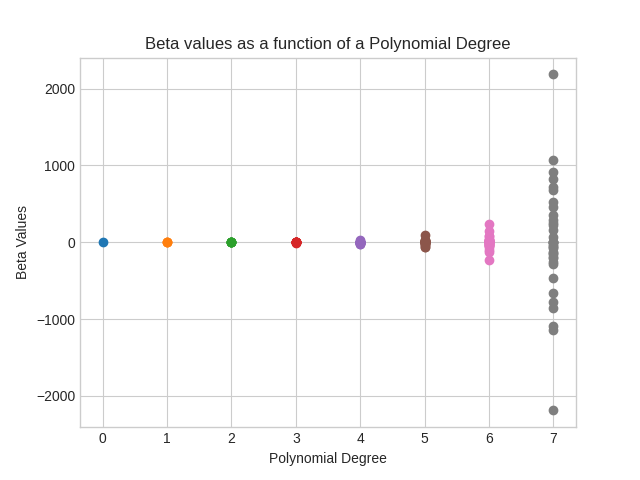
\includegraphics[width=15cm]{Images/beta_ols.png}
     \caption{Betavalues for OLS with uniform data. We can see that the beta values diverge when the polynomial degree increase. Each color represents betavalues for one degree.}
     \label{fig:betavalues_ols}
\end{figure}

Moving on to the results for the Ridge regression, we observe the MSE and $R^{2}$ scores (Figure \ref{fig:ridge mse}). The seven different lambdas are all equal from degree 0 to degree 1, but diverges after that for both MSE and R2. It is clear that the lower the lambda values, the better the Ridge regression model fits this data. Lower lambdas than 1e-05 did not improve the model further, while adding more degrees after nine only improved the performance by negligible amounts. 

\begin{figure}[H]
     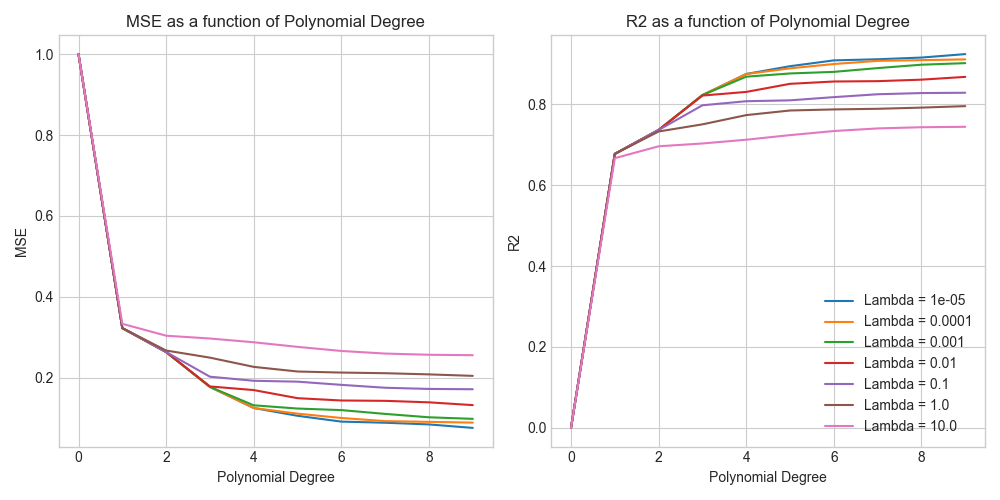
\includegraphics[width=15cm]{Images/ridge_error_degree.png}
     \caption{Performance of Ridge as a function of polynomial degree for different lambdas. On uniform data we see that lambda 1e-05 gives the best performance.}
     \label{fig:ridge mse}
\end{figure}

The results from Lasso regression in Figure \ref{fig:lasso mse} show more variability compared to Ridge. The lambda value of 1e-06 performs best up to degree 5, except for degree 4, and again at degree 8 before overfitting occurs. Lambda 1e-05 performs best for most other degrees, with the exception of degree 4, where 1e-04 is optimal. Overall, 1e-05 appears to be the most stable. We observe that at lower complexities, smaller lambda values perform best. However, as complexity increases, slightly larger lambda values yield the lowest MSE, while the smallest lambdas drop in performance. This happens because larger lambdas strike a better balance between capturing data nuances and avoiding overfitting. \cite{openai2023chatgpt}

\begin{figure}[H]
     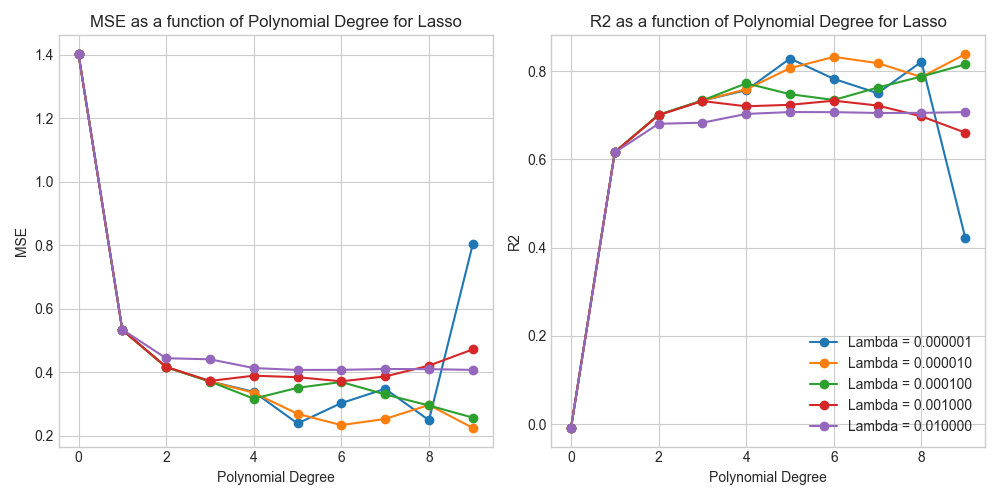
\includegraphics[width=15cm]{Images/lasso_error_degree.png}
     \caption{Performance of Lasso as a function of polynomial degree for different lambdas. On uniform data we see that lambda 1e-05 is performing best.}
     \label{fig:lasso mse}
\end{figure}

When comparing the three regression methods it seems that Ridge is performing best overall, with the lowest MSE and the highest R2 values. It is also the most stable method as the performance increases in proportion to the complexity. We believe Ridge is better than Lasso because the spesific dataset we used is too simple and too small for the more complex Lasso penalty to show it's potential. However, the OLS model overfits the data, so a penalty is beneficial. 

\subsubsection{Bootstrap: bias variance tradeoff}

As we don't have the computational power to show the bias-variance tradeoff for the real data, we present the bootstrap analysis for the synthetic data. We can see from Figure \ref{fig:bootstrap1000samples} that the bias is decreasing as a function of model complexity. In contrast, the variance is increasing with model complexity. As the error can be decomposed to bias and variance, we want to find the optimal balance between the bias and the variance. From our error plots we expected the optimal bias variance tradeoff to be somewhere after degree 8. We observe that it is between degree 10 and 11. For the optimal bias variance trade off, we would choose degree 11. 

\begin{figure}[H]
     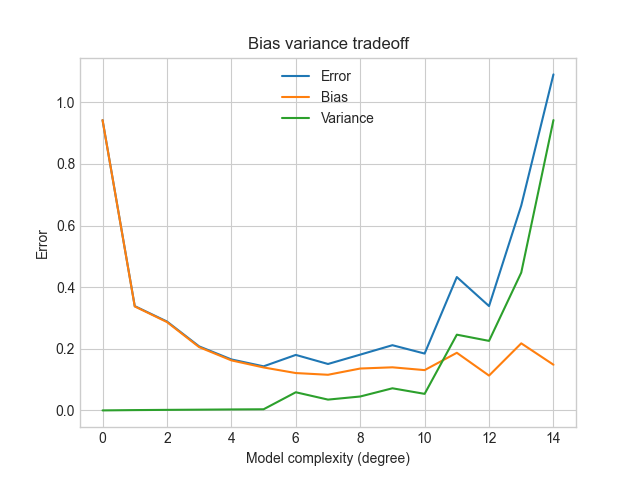
\includegraphics[width=15cm]{Images/uniform_1000_bootstrap.png}
     \caption{Bootstrap of uniform data with 1000 samples (we had to increase the number of samples to see the trade-off) and 100 bootstraps. We can clearly see the bias variance tradeoff at the crossing point between degree 10 and 11.}
     \label{fig:bootstrap1000samples}
\end{figure}

\subsubsection{Comparison of OLS, Lasso and Ridge on terrain data}

One main finding is that our Lasso model, which produced decent recults with a small sample from the uniform distribution, requires a significant amount of computational resources with the high dimensional terrain data. We adjusted the hyperparameters that could affect runtime and tested both locally and on a remote machine, but were not successfull in producing sensible results. However, we can see in Figure \ref{CV_terraindata} that Ridge and Lasso have the most stable performance  with increasing polynomial degree. OLS on the other hand have a rapidly increasing MSE after degree 5. 

\begin{figure}[H]
     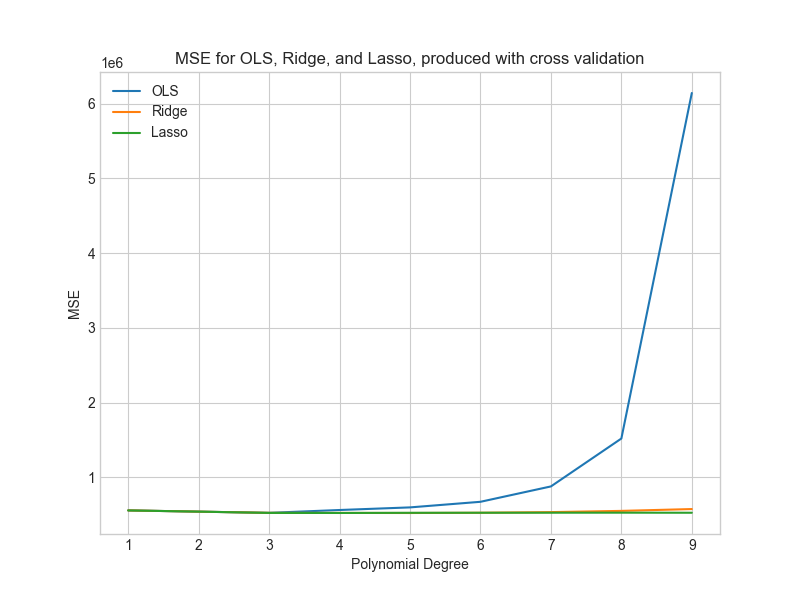
\includegraphics[width=\textwidth]{Images/CV_terrain_data.png}
     \caption{MSE after cross validation showing that OLS is least stable in increasing model complexity. The plot is based on terrain data.}
     \label{CV_terraindata}
\end{figure}

Because Lasso was the best performing model on the terrain data in terms of producing stable results with increasing complexity, we decided to compare the heatmap of the terrain data in Figure \ref{terrain data heatmap comparison} and the reproduction from Lasso in Figure \ref{fig:Lasso CVHeatmap} using cross validation. We were hoping to be able to recreate some of the terrain data, but we can see that the reproduction doesn´t capture the terrain data, only the gradient shadow. This is supported by the relatively high MSE. It should again be noted that because of the lack of computational resources we are not able to explore the increase of model complexity, which is a weakness with the comparison. In Appendix A we have included heatmaps in Figure \ref{fig:four graphs} for the three regression methods computed without cross validation to show that it is possible to get better reproductions on this data, but not without overfitting it. 

\begin{figure}[H]
     \begin{subfigure}[h]{0.45\textwidth}
         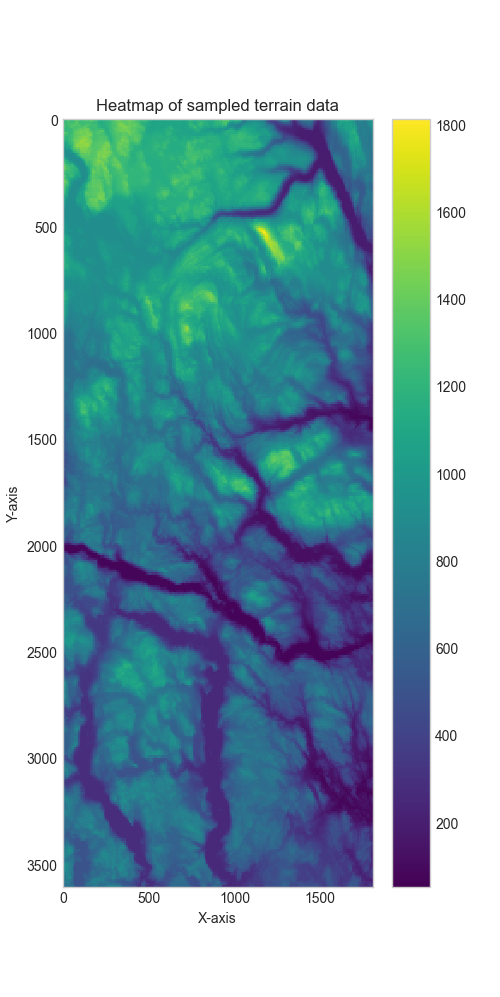
\includegraphics[width=\textwidth]{Images/sampled_data_heatmap.png}
         \caption{Original sampled data}
         \label{terrain data heatmap comparison}
     \end{subfigure}
     \hfill
     \begin{subfigure}[h]{0.45\textwidth}
         \centering
         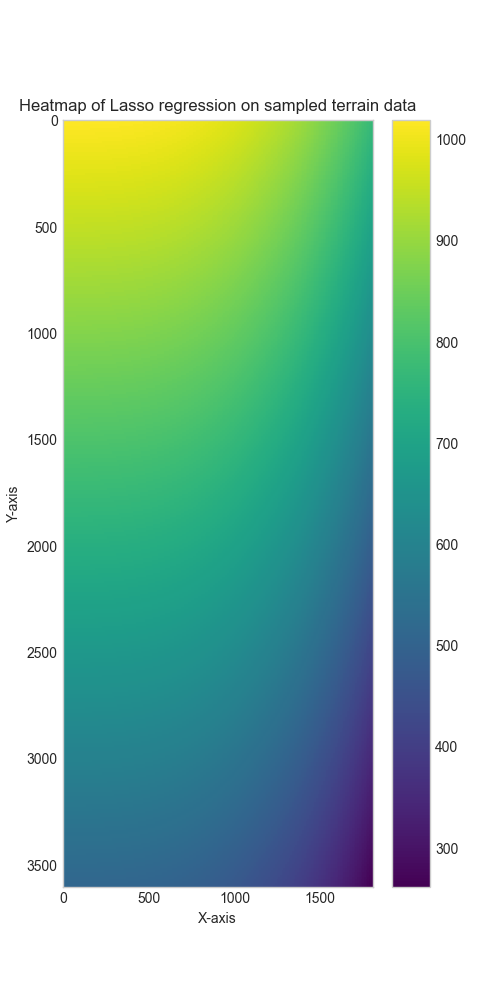
\includegraphics[width=\textwidth]{Images/cv_lasso_terrain_heatmap.png}
         \caption{Lasso}
         \label{fig:Lasso CVHeatmap}
     \end{subfigure}
     
        \caption{Heatmaps showing the true terrain side by side with the terrain estimated by the Lasso model. The Lasso model is chosen through cross validation. We see that by emphasizing that it should generalize to new data, it is not able to recreate our original terrain data.}
        \label{fig:four graphs}
\end{figure}



% ===========================================
\newpage
\section{Conclusion}\label{sec:conclusion}
%
\label{sec:conclusion}
In conclusion, this study provides a comparison of three linear regression techniques: OLS, Ridge, and Lasso, applied to both synthetic and real-world high-dimensional terrain data. The results demonstrate that Ridge regression consistently performs best across various polynomial degrees and regularization parameters on synthetic data from the uniform distribution. When switching to terrain data, Lasso performs best across the different conditions, although it was limited by the computational resources. OLS, while simpler, performed similar to the others when restricting the models to less features, highlighting that model complexity does not always guarantee better performance. The study underscores the importance of careful hyperparameter tuning and model selection, which should be based on the nature of the data and computational resources. Future work should focus on refining these models by leveraging more computational power and exploring higher degrees of model complexity, especially for real-world data applications.


% ===========================================
\newpage
 \section*{Appendix A}\label{sec:AppendixA}
%
\label{sec:appendix}
\begin{figure}[H]
     \begin{subfigure}[h]{0.23\textwidth}
         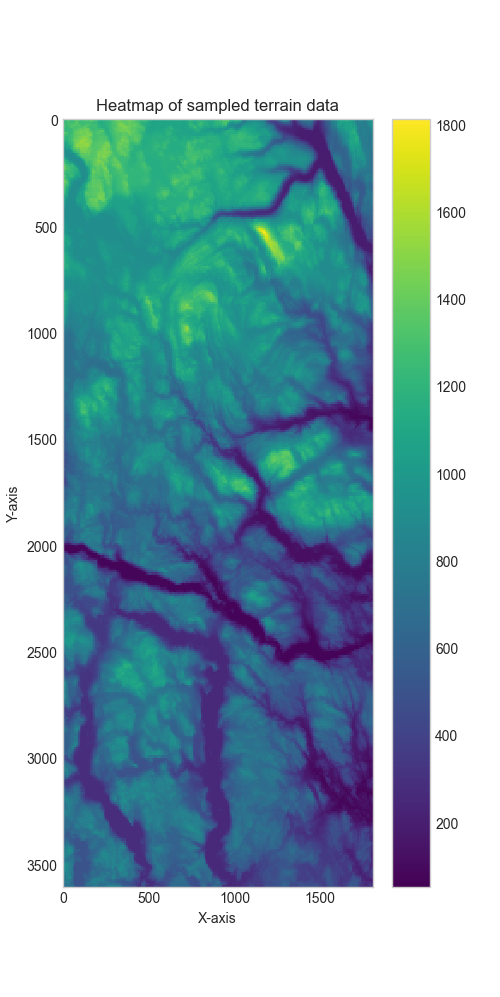
\includegraphics[width=\textwidth]{Images/sampled_data_heatmap.png}
         \caption{Original sampled data}
         \label{terrain data heatmap}
     \end{subfigure}
     \hfill
     \begin{subfigure}[h]{0.23\textwidth}
         \centering
         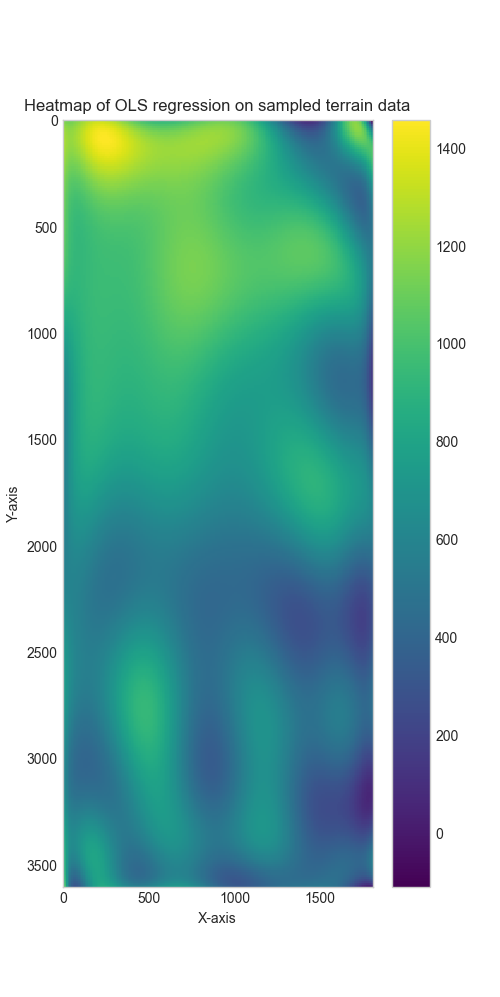
\includegraphics[width=\textwidth]{Images/ols_terrain_heatmap.png}
         \caption{Ordinary least squares}
         \label{fig:ols heatmap}
     \end{subfigure}
     \hfill
     \begin{subfigure}[h]{0.23\textwidth}
         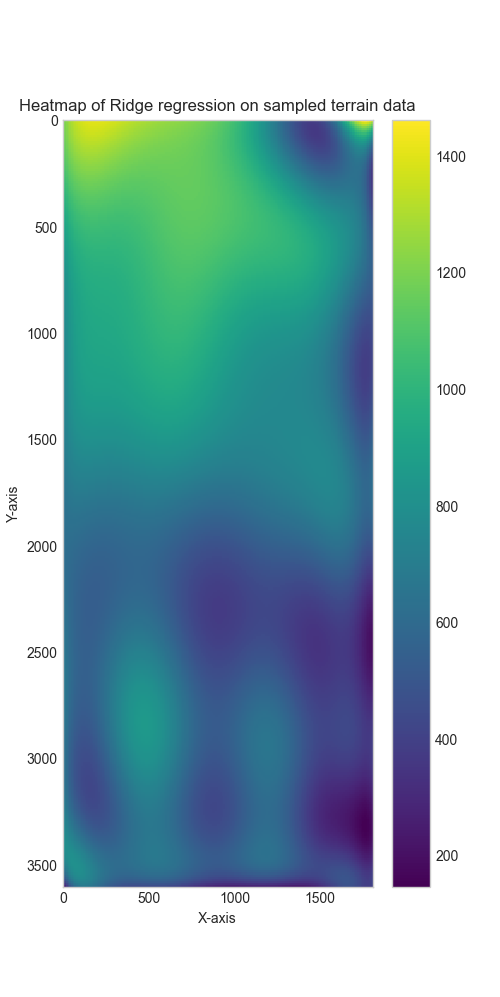
\includegraphics[width=\textwidth]{Images/ridge_terrain_heatmap.png}
         \caption{Ridge}
         \label{fig:ridge heatmap}
     \end{subfigure}
     \hfill
     \begin{subfigure}[h]{0.23\textwidth}
         \centering
         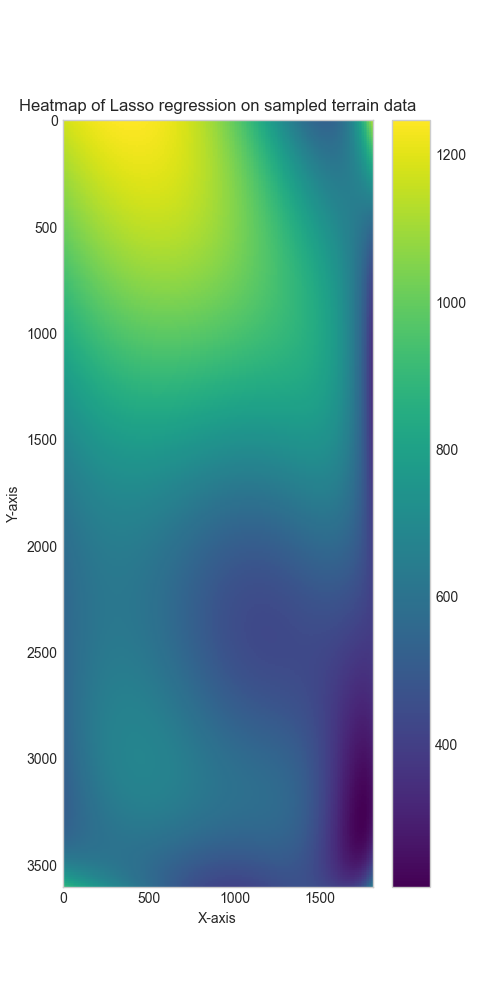
\includegraphics[width=\textwidth]{Images/lasso_terrain_heatmap.png}
         \caption{Lasso}
         \label{fig:lasso heatmap}
     \end{subfigure}
        \caption{Heatmaps showing the true terrain side by side with the estimated terrain of OLS, Ridge and Lasso without cross validation. We see that the predictions is most precise with OLS, less precise with Ridge, and most blurry with Lasso.}
        \label{fig:four graphs}
\end{figure}


When plotting our results in figure \ref{fig:lasso heatmap}, found in appendix A, in a heatmap, we see that it is able to reproduce some of the structures in the original data, but the result is blurry compared to that of Ridge and OLS. 

% An appendix can be useful if there are details you want to include that do not fit in the main text. But if you include an appendix, make sure to explicitly refer to it somewhere in the main text.


% ===========================================
\onecolumngrid

\clearpage

\section*{References}
\bibliographystyle{unsrt}
\bibliography{bibliography.bib}


\end{document}
